\chapter{Theory}
\label{chap:theory}

% -------------------------------------------------------------------------------------------------
%                                            Structure
% -------------------------------------------------------------------------------------------------

% - Reiteration of Idea       -> Was wird hier gemacht    -> Was benötigt man dafür

% - Impl Platform             -> Was provided die Hardware und Plattform schon, Was braucht es noch?

% - Implementation Steps      -> Overview over the implementation chapter (but without the single address cases)

% -Übersicht über die benötigten Änderungen
%     - TLB Miss Exception
%         - Exceptions and TLBS in RISC-V
%         - New Exception
%         - Vorlage: MIPS
%             - Riscv Exception basics (if not in fundamentals)
%             - New Exceptions? -> Was man beachten muss


%      - Exception Handler in general
%             - General Stuff, xv6 Exception Handler
%             - Vectored
%             - All registers that come into play
%             - xv6 book, exception machinery

%         - Exception Handler for the TLB Miss exception

%     - TLB Filling
%         - Vorlage MIPS

%         - RISCV CSRs -> Extensibility


%         - QEMU TLB


%         - Concrete CSRs for TLB filling (THIS IS THE RESULT OF THIS CHAPTER)
%             (- TLB Flushing, Replacement policy (vs mips))


%     - Mapping functions
%         - Segmented
%         - More?


% -------------------------------------------------------------------------------------------------
%                                            Intro
% -------------------------------------------------------------------------------------------------
% Überblick über die Idee schaffen -> Virtueller Speicher durch funktion möglich


This chapter presents the theoretical foundation of the the implementation presented in the next chapter.\\
It will start with a short elaboration on the general idea followed by a description of the
programming platform.\\
It then presents the theory behind the different components of the implementation.
% Then?

% -------------------------------------------------------------------------------------------------
%                                            Idea
% -------------------------------------------------------------------------------------------------
% Beantwortet die Frage: Was wird hier überhaupt gemacht? (Ohne zu sehr ins detail zu gehen)
% Auch die Motivation und was das Ergebnis sein könnte/ erwartet ist



\section{General idea of stateless Virtual Memory}
% Idea Description

% The implementation is not only about the mapping functiion but also about the  platform modifications to create mapping functions

The goal of this work is to provide a proof of concept of an alternative approach
to virtual memory management that reduces the overhead associated with traditional page tables walks.\\
Instead of suffering the penalty of up to five memory accesses on a TLB miss,
we want to explore using simple functions for the mapping.

Figure \ref{fig:theory:normal_tlb_miss} shows the usual architecture of a system
with a hierarchical page table.\\
This architecture provides only limited flexibility in interacting with the TLB, especially when it comes to TLB writes.\\
Architectures like MIPS allow direct manipulation of TLB structures and thus provide a good framework for implementing new approches for virtual memory management.\\

The architecture is only one half of the design. To test the ideas for mapping
functions, a system utilizing the memory system and defining the functions is also necessarry.\\
The xv6 educational operating system provides a good platform for experimentation as it is very lightweight and provides a Unix-like interface and structures.\\

xv6 is designed for RISC-V, but RISC-V does not allow for flexible software-management of the TLB structure.\\
Thus part of this chapter will describe the theoretical foundations for modifying
the QEMU/RISC-V emulator to transform the memory system architecture to something
more similar to MIPS.\\
The final architecture for the memory sytem will look like depicted in figure \ref{fig:theory:mapping_fx}
% TODO der Zwischenschritt mit dem Software Page Table walk wird dann in der Impl
% eingeführt

% Normal Page Table Walk
\begin{figure*}[ht!]
    \centering
    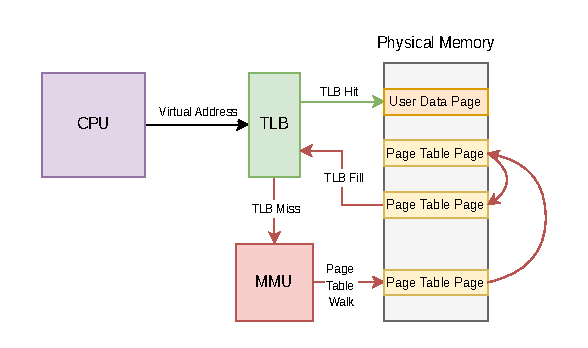
\includegraphics[scale=1.5]{figures/theory_normal_tlb_miss.pdf}
    \caption[Usual TLB Miss]{This figure shows what usually happens when the TLB misses:
        the miss will invoke the hardware state machine page table tree walker; the walker traverses
        the page table tree and if a valid PTE is found, the mapping is added to the TLB. The processor
        then executes the failing instruction again which will then result in a TLB hit}
    \label{fig:theory:normal_tlb_miss}
\end{figure*}
% Virtual Memory using a Mapping Function
\begin{figure*}[ht!]
    \centering
    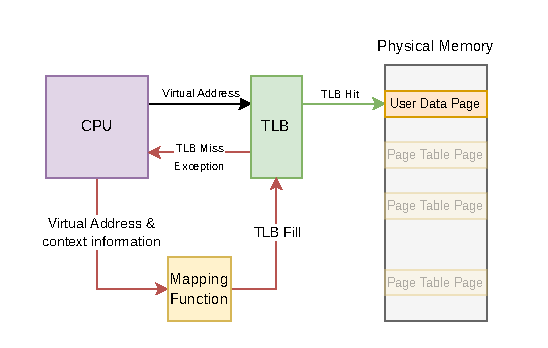
\includegraphics[scale=1.5]{figures/theory_mapping_fx.pdf}
    \caption[Virtual Memory using a mapping function]{Instead of emulating a hardware page table walk in software on
        a TLB Miss exception, a mapping function is invoked that calculates the PTE using arithmetic primitives and tries
        to avoid memory references.}
    \label{fig:theory:mapping_fx}
\end{figure*}

% TODO %%%%%%%%%%%%%%%%%%%%%%%%%%%%%%%
% Give a rough description of the required changes here?
%%%%%%%%%%%%%%%%%%%%%%%%%%%%%%%%%%%%
% Overview of the different parts necessary to implement the idea
\section{Conceptual Basis for Implementation Modifications}
% What to do to realize this idea? (basically top level overview of the theory and impl chapters)
Dieser Abschnitt enthält die theoretischen Ausarbeitungen zu den einzelnen Bestandteilen die für
die Implementation des Software kontrollierten TLB Miss Handlers benötigt werden. Diese Bestandteile
sind wie folgt:
\begin{itemize}
    \item Die Erweiterung des Qemu Emulators um einen Exceptionwurf bei TLB Miss
    \item Einen Maschine-Mode Traphandler in xv6 der die neue TLB Miss Exception entsprechend behandelt
    \item Eine Möglichkeit um TLB einträge mittels spezieller Instruktionen zu schreiben
\end{itemize}

% -------------------------------------------------------------------------------------------------
%                                            Required Changes
% -------------------------------------------------------------------------------------------------

% What to do to realize this idea? (basically top level overview of the theory and impl chapters)
% New Exception - TLB Miss Exception
% CSRs to write TLBs
% Exception Handler

% Steps necessary to implement Idea -> relating to the implementation

% Architecture: Handle TLB Miss -> Like Liedtke MIPS

% TLB Exception
% TLB Filling



%elaboration on general costs of page table walks -> basically exactly what related
% work motivated their designs with



\todo{elaboration on xv6 here or in fundamentals (or an extra platform chapter)?? -> because theory
    may be independent from the platform in big parts, but still needs to be taken into consideration (like with
    csrs)}

% TODO %%%%%%%%%%%%%%%%%%%%%%%%%%%%%%%
% Kapitel endet mit der Frage was man für die Implementation benötigt?

% -------------------------------------------------------------------------------------------------
%                                            Platform
% -------------------------------------------------------------------------------------------------
% Answers: Welche Platform wird verwendet? Warum?  Was provided die Platform, was nicht?
\section{Platform}
The chosen platform is the xv6 operating system \cite{xv6source}. It is a teaching operating system
used by some MIT courses.\\
xv6 implements the basic Unix Version 6 interfaces, but does so in a very simplified fashion.\\
There is a x86 version and a RISC-V version. For this project, the RISC-V version was chosen.\\
xv6's simplicity and the accompanying handbook \cite{cox2011xv6} make it a good choice for a first
proof of concept.

xv6 will be run on the QEMU \cite{QEMUSource2024} emulator. The QEMU RISC-V emulator implements
all the RISC-V features and extensions that xv6 needs.

Running the operating system on an emulator is a necessity, because the requires the hardware to
throw a TLB Miss exception.\\ The RISC-V ISA does not provide such functionality by default, so
part of the theory and implementation chapters will be dedicated to extending the RISC-V ISA and
the QEMU emulation to support TLB Miss exceptions.
%Implementation Platform
Diese Kapitel betrachtet zwar nur die Theorie des softtlb desings, allerdings muss diese in Kontext
der gewählten Platform gestellt werden und wird daher an manchen Stellen in tieferes Detail der konkreten
Platform eintauchen als man für eine theoretische Ausarbeitung des Designs erwarten würde.
Das ist wichtig um dem späteren Implementierungskapitel den nötigen Kontext zu liefern.\\
Als Platform für die Implementierung wurde der Einfachkeit halber das xv6-riscv educational operating
system \cite{cox2011xv6} gewählt.\\
\textit{Xv6} wird am MIT genutzt um Operating Systems Kurse zu bieten und bietet mit dem Handbuch eine
einfache und verständliche Platform die ein vereinfachtes Unix Version 6 Interface implementiert.\\
Xv6 gibt es in einer x86 version und in einer RISC-V version, es wurde hier die RISC-V version verwendet.
\\
Da im Rahme der Implementierung einer neuen Exception das nutzen echter RISC-V Hardware nicht möglich
ist, muss ein Emulator benutzt werden um die nötigen Änderungen an der ISA zu implementieren und zu nutzen.
Dafür wurde der Qemu Emulator gewählt, da dieser sehr Umfassend und performant ist und außerdem einen
TLB emuliert.
% Zukünftige Idee -> Configurierbarer "stateless" physical frame calculator hw baustein

% Was provided die Platform noch nicht, was muss noch gemacht werden um das Design zu realisieren?
% Implications of programming platform on implementation -> needing to implement TLB Miss
% -------------------------------------------------------------------------------------------------
% -------------------------------------------------------------------------------------------------
%                                            IMPL THEORY
% -------------------------------------------------------------------------------------------------
% -------------------------------------------------------------------------------------------------


% -------------------------------------------------------------------------------------------------
%                                            TLB MISS EXCEPTION
% -------------------------------------------------------------------------------------------------
% -------------------------------------------------------------------------------------------------
\section{TLB Miss Exception}
Usually, an operating system running on RISC-V hardware is not notified directly of TLB misses.
A TLB miss can only be infered when a page fault occurs. Otherwise, TLB misses will be handled
by the MMU.\\
To manage a TLB in software the operating system needs to be made aware that a TLB miss occured.\\
The natural mechanism to do this is the exception mechanism. \todo{similarity TLB Miss Page Fault}

% -------------------------------------------------------------------------------------------------
\textbf{RISC-V Exceptions}
Unlike MIPS \cite{heiserAnatomyHighPerformanceMicrokernel}, RISC-V does not raise a TLB miss exception
on TLB miss.\\
Instead, the \emph{Virtual Address Translation Process} is initiated: The MMU will walk through
the page table tree and may, depending on the PTEs, either throw different kinds of page faults, or
successfully add the missing entry to the TLB.\\
At this point the faulting instruction will either be repeated, if the TLB fill was successful, or
a page fault exception will be invoked. The kernel then has to handle that page fault with help
of the contents of the \texttt{satp} and \texttt{mtval} (or \texttt{stval}) registers.

The behavior of a TLB Miss exception should be pretty similar: If the TLB hits, the program will
just continue as usual. If the TLB misses, a exception should be risen, providing context
information about the miss in registers. The invokation of the hardware page table walker is
not necessary.


% -------------------------------------------------------------------------------------------------
\textbf{Adding a new Exception to RISC-V}
Extending the emulator to throw a new exception is explained in the Implementation chapter.
On the theoretical side, it is important to chose a exception code from the code ranges designated
for custom use. These are $24-31$ and $48-63$ \cite{RISCVInstructionSet}. For the implementation we chose $24$ or $0x18$.



% -------------------------------------------------------------------------------------------------
%                                            Exception Handling
% -------------------------------------------------------------------------------------------------

% -------------------------------------------------------------------------------------------------
\section{Exception Handling}
Throwing a exception is only one half of the puzzle. The operating system also has to handle the exception
properly.
% -------------------------------------------------------------------------------------------------
\subsection{L4/MIPS TLB Exception Handling}
MIPS vectors its exception vectors in a continuous area in memory, starting at a base address.
That gives the TLB miss handler 32 instructions to server the TLB Miss. Otherwise it has to jump
somewhere with more space.\\
The \emph{Fast TLB Miss} handler is able to service the miss using only the two kernel-reserved
registers \texttt{k0} and \texttt{k1} and another register, which has to be saved first \cite{heiserAnatomyHighPerformanceMicrokernel}.\\
Thus the memory footprint of handler is really low.

% -------------------------------------------------------------------------------------------------
\subsection{xv6 Exception Handler}
xv6's exception handler does not actually handle most of the exceptions. For most of the exceptions,
but notably also the different page fault exceptions, xv6 will simply kill the offending process \cite{cox2011xv6}.

% -------------------------------------------------------------------------------------------------
\subsection{TLB Miss Exception Handler}
To simplify things, we will let the TLB Miss exception handler run in machine mode only.
The usual mode for a operating system kernel would be the supervisor mode. However, this
mode also uses address translation. This could create a situation in which we would have
to deal with nested exception.\\

\textbf{Catching the Exception} M-mode exceptions will set the program counter to the address
specified in the \texttt{mtvec} register. Originally, xv6 only serviced the asynchronous
timer interrupt in machine mode. Every other trap is forwarded to supervisor mode.\\
The trap vectoring mode can also be changed by setting the \texttt{MODE} field of the
\texttt{mtvec} register \cite{RISCVInstructionSet}. The alternative mode forwards
each interrupt to its own address, set at a fixed offset from the \texttt{BASE} address.
\todo{mtvec bytefield}.

Every exception will still be forwarded to the \texttt{BASE} address set in the \texttt{mtvec}
register, regardless of the vectoring mode.

The value of the \texttt{mcause} register identifies the reason for the exception.
This value can be used in something like a switch-case statement to call specific handlers
for the different exception causes.
This switch-case is not really necessary in xv6, since the only exception that can enter
the machine-mode exception handler is the TLB Miss exception.

Before running any code that modifies general-purpose registers, the current state of the
registers and the program counter should be saved to memory. These need to be restored after
the exception handler code has finished.\\
This is essential to keep the process, that was just running when the exception triggered,
in an consistent state when execution resumes.

% Catching New Exception
%   Current xv6 machine mode exception handler ( -> maybe too implementation specific)
%   riscv interrupt mechanism (precice, vectorized)
%   Exception Catching theory, context switch, state save restore



% -------------------------------------------------------------------------------------------------
%                                            TLB FILLING
% -------------------------------------------------------------------------------------------------
\section{TLB Filling}
Not only does the operating system need to be made aware of TLB misses,
the operating system also needs to be able to write to the TLB to actually create
mappings that will be used after the handler finishes.\\
RISC-V also does not provide any means to write to the TLB out of the box. But the RISC-V Control and Status Registers
(CSRs) allow for a great deal of extensibility \cite{riscvreader}.
With CSRs, it is possible to implement custom behavior, which can then be accessed using instructions
of the \texttt{CSRR}\todo{check reader: is this correct?} instruction group.\\
To make an informed decision on how the CSR format for TLB writing may look like, we will first
look at the TLB and the TLB instructions of \emph{MIPS}. Then we will take a look at what the
RISC-V ISA specifies about TLB, how QEMU implements TLBs and finally we will look at a the
CSR format that is used for the implementation.

% -------------------------------------------------------------------------------------------------
\subsection{MIPS TLBs}               % Combine TLB Sections into one ( Multiple TLB designs clash here ...)

%       Starting with MIPS for inspiration on how instructions for TLB manipulation may look like
%       Then continue with a possible RISCV Implementation Idea
%       I-TLB and D-TLB out of scope
% Inspiration: MIPS

The MIPS64 instruction set manual \cite{MIPSArchitectureProgrammers2016}
shows a number of different instructions concerned with the invalidation, probing, flushing, reading
and writing (indexed and random).\\
The most interesting instruction for a first design would be the \texttt{TLBWR} instruction for writing a TLB
entry at a random index. With a similar instruction in RISC-V, we can already implement a purely
software-controlled virtual memory system.\\
The other types of TLB instructions that MIPS provides are not strictly necesarry,
except for flushing. Without being able to flush existing translations from the TLB,
user mode processes may try to access physical mappings stemming from other processes.\todo{can this even happen? -> why else would we need to flush the tlb??}
But the RISC-V priviledged Architecture already provides this functionality
with the \texttt{sfence.vma} instruction \cite{riscvreader}.\\


% Replacement policy
%   MIPS -> Indexed writes
A advantage of software-managed TLBs is, that the operating system can implement custom
TLB replacement policies, that may even change depending on workload, programs running
and other circumstances.\\
The default replacement strategy for the MIPS \texttt{tlbwr} instruction is to simply
use the value of the \texttt{C0\_RANDOM} register as the index for the next TLB entry
to be replaced. The name of that register is missleading, because it is not actually a
random value, but it is rather decremented on each instruction\cite{heiserAnatomyHighPerformanceMicrokernel}.\\
It is not clear whether this is a sensible replacement strategy,
but it can be used to ensure that the same TLB slot is not used for every \texttt{tlbwr} if the implementation
does not provide for any further replacement strategy.\\
Some TLB entries can be protecte from this ''random'' replacement by setting a value in the \texttt{C0\_WIRED}
register. The value in this register represents a lower bound, protecting all TLB entries that lie below it.\\
This is useful to keep some mappings in the TLB that are valid all the time.

% TODO should this be here? We should probably have a discussion about xv6 first
%Protected TLB entries in xv6 -> Trampoline page
Having a protected space of TLB entries can especially be useful for global mappings. xv6 employs such a global
mapping for every process and the kernel with the trampoline page.\todo{trampoline page should be explained in fundamentals/platform}

\paragraph{MIPS - TLBWR} The arguments for the instruction need to be written in some
other registers - \texttt{EntryHi}, \texttt{EntryLo0}, \texttt{EntryLo1} and \texttt{PageMask}.


% -------------------------------------------------------------------------------------------------
\subsection{RISC-V TLBs}
% Riscv can flush entries of a specific ASID only, this means that it keeps that information
% selective TLB flushing -> RISCV ASIDs (or even no TLB flushing  because VAs contain ASID?)
% Somewhere in the TLB structure
\subsection{QEMU TLBs}
% Qemu -> TLB structure, replacement
RISC-V and its extensions currently provide no support for modifying the TLB in software.
RISC-V does however provide a lot of extensibility with the \texttt{Control and Status Registers} (CSRs).\\
CSRs are part of the RISC-V priviledged architecture and are provided by the \texttt{Zicsr} extension\cite{RISCVInstructionSet}.\\

% How is the RISCV Tlb indexed -> Check Qemu source

% -------------------------------------------------------------------------------------------------
\subsection{RISC-V CSRs}
% CSR size
% -------------------------------------------------------------------------------------------------
\subsection{TLB CSRs}
The minimum information the hardware needs to create a mapping is the faulting physical address and
the virtual address it maps to.\\
The mapping is has a granularity of 4 KB pages. Thus the lower 12 bits of both the physical and the
virtual address are not needed.\\
This still leaves $2*(64-12)=104$ bits for the mapping.\\
The virtual address can not be easily shortened anymore. Taking some of the most significant bits
would shorten the virtual memory space of the programs.\\
The physical address could still be shortened to only have enough bits to cover the physical address
space used by xv6.\\
But this would still end up taking more than 64 bit and thus more than one CSR.

So instead of trying to save as much space as possible, two CSRs are used.\\
They are called \texttt{tlbwh} (TLB Write High) and \texttt{tlbwl} (TLB Write Low).
The emulator will expect the physical address \ref{fig:theory:sv39pa} in \texttt{tlbwh} and a the virtual address in form
of a PTE \ref{fig:theory:sv39pte} in the \texttt{tlbwl} CSR.
% Fixed TLB format, but flexibilty of CSR format




\todo{TLB CSR Format}

\todo{Hardware dependenc -> still dependent on the TLB structure of RISCV Sv39, VAs and PAs remain, as do PTEs}



% -------------------------------------------------------------------------------------------------
%                                            MAPPING FUNCTION
% -------------------------------------------------------------------------------------------------
\section{Mapping Functions}
% -------------------------------------------------------------------------------------------------
\subsection{Segmented Mapping}

\cite{tanenbaumOS}
The first attempt at a stateless \todo{Begriff an sinnvoller stelle einführen} paging design
uses a design that determines memory allocation at compile time.
% Assumptions
%Design of Segmented VM softtlb -> Assumption: Process Memory allocation Model -> Only growing upwards
% Segmentation -> ASIDs -> HW support for Address Space Protection
% -> [jacob1998virtualissues]


% A look at input and output data
% Calculation of addresses

% xv6 Perspective and specifcs (but still theory!) -> Into Impl?
%   Special mappings -> special case in tlb manager (e.g. Trampoline)

% End of Theory: A simple mapping function - TLB Manager
%   TODO What does the reader need to know at this point, e.g. what does need to be decided
%   in theory to create a TLB Miss Handler design??

% xv6 Process Memory Model
The new memory system needs to be compatible with the existing one. Otherwise the way xv6
user processes are built and structures needs to be changed.\\
The program memory model of xv6 programs is shown in figure \ref{impl:xv6layout}

\begin{figure*}[t!]
    \centering
    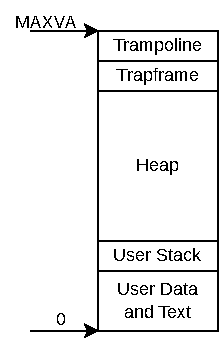
\includegraphics[scale=.5]{figures/prog_vm.pdf}
    \caption[xv6 memory layout]{Virtual memory layout of xv6 processes. Taken from the xv6 book \cite{cox2011xv6}.}
    \label{impl:proclayout}
\end{figure*}

Xv6 processes have their data and text segment and the stack at the very bottom of the virtual
address space \cite{cox2011xv6}.\\
A peak into the implementation of the \texttt{sbrk()} system call also shows us, that the heap
address space grows linearily from low to high addresses.\\
None of the xv6 programs differ from this memory model. There are no pages mapped in the
middle of the address space.\\
The only special cases are the \textit{trampoline} and \textit{trapframe} pages.
\todo{trampoline and trapframe already explained?}

% Segmented memory layout

\begin{figure*}[ht!]
    \centering
    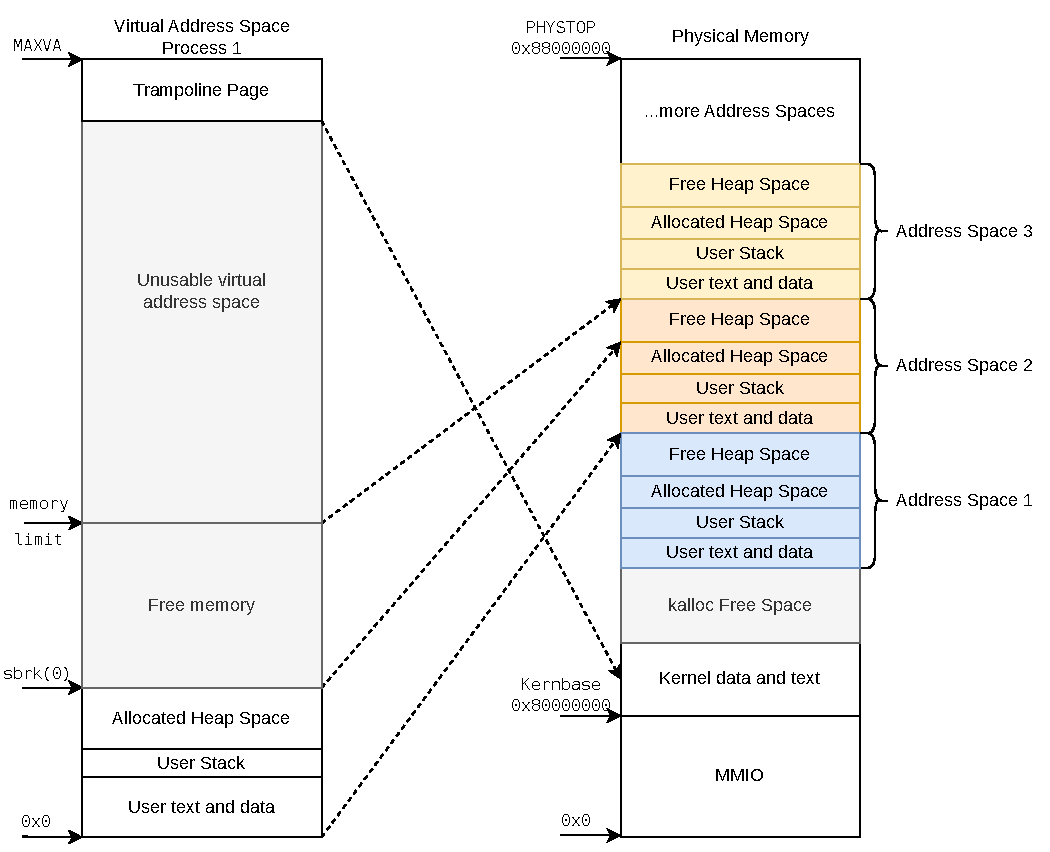
\includegraphics[]{figures/segmented_layout.pdf}
    \caption[Segmented Memory Layout]{\textbf{Segmented Memory Layout}}
    \label{fig:theory:segLayout}
\end{figure*}


% -------------------------------------------------------------------------------------------------
% -------------------------------------------------------------------------------------------------
% -------------------------------------------------------------------------------------------------
% -------------------------------------------------------------------------------------------------
